\Opensolutionfile{ans}[ans/ansCD2D1-5]
\begin{dang}{Sự tương giao của hai đồ thị}.
\end{dang}
\paragraph{Các ví dụ}
\begin{vd}%[2D1Y5-4]%Ví dụ 1.
	Tìm tọa độ điểm $I$ là giao điểm của đồ thị hàm số $y=4x^3-3x$ với đường thẳng $y=-x+2$. 
	\choice
	{\True $I(1,1)$}
	{$I(2,1)$}
	{$I(2,2)$}
	{$I(1,2)$}
	\loigiai{
		Xét phương trình hoành độ giao điểm $4x^3-3x=-x+2\Leftrightarrow x=1$.\\
		Suy ra tọa độ điểm $I(1,1)$.}
\end{vd}
\begin{vd}%[2D1Y5-4]%Ví dụ 2.
	Đồ thị hàm số $y=15x^4-3x^2-2018$ cắt trục hoành tại bao nhiêu điểm?
	\choice
	{$1$ điểm}
	{$3$ điểm}
	{$4$ điểm}
	{\True $2$ điểm}
	\loigiai{
		Số giao điểm của đồ thị hàm số với trục hoành là số nghiệm của phương trình: $15x^4-3x^2-2018=0 \quad (1)$.
		Đặt $t=x^2, t\geq 0$, phương trình trở thành: $15t^2-3t-2018=0 \quad (2)$.\\
		Vì phương trình (2) có $a \cdot c<0\Rightarrow$ phương trình (2) có $ 2 $ nghiệm trái dấu\\
		$ \Rightarrow $ phương trình (1) có hai nghiệm phân biệt.\\
		Vậy đồ thị hàm số đã cho cắt trục hoành tại hai điểm phân biệt.}
\end{vd}
\begin{vd}%[2D1K5-4]%Ví dụ 3.
	Cho hàm số $y=\dfrac{2x-1}{x-1}$ có đồ thị $(C)$. Tìm tất cả các giá trị của tham số $m$ để đường thẳng $d\colon y=x+m$ cắt $(C)$ tại hai điểm $A,B$ phân biệt sao cho $AB=4$. 
	\choice
	{$m=-1$}
	{$\hoac{&m=0\\&m=3}$}
	{\True $\hoac{&m=-1\\&m=3}$}
	{$m=4$}
	\loigiai{
		$d$ cắt $(C)$ tại hai điểm phân biệt $\Leftrightarrow\dfrac{2x-1}{x-1}=x+m$ có hai nghiệm phân biệt\\
		$ \Leftrightarrow 2x-1=(x-1)(x+m) $ có hai nghiệm phân biệt khác $1$ \\
		$ \Leftrightarrow x^2+(m-3)x+1-m=0 \quad (1)$ có hai nghiệm phân biệt (do $ x =1 $ không thỏa mãn phương trình)\\
		$ \Leftrightarrow\Delta=(m-3)^2-4(1-m)>0\Leftrightarrow m^2-2m+5>0 $ luôn đúng.\\
		Khi đó $A(x_1;x_1+m), B(x_2;x_2+m)$ với $x_1,x_2$ là các nghiệm của (1).\\
		Theo Vi-ét: $\heva{&x_1+x_2=3-m\\&x_1x_2=1-m.}$ \\
		$AB=\sqrt{(x_2-x_1)^2+(x_2-x_1)^2}=\sqrt{2\left[(x_1+x_2)^2-4x_1x_2\right]} =\sqrt{2\left(m^2-2m+5\right)}=\sqrt{2(m-1)^2+8}$.\\
		$AB=4\Leftrightarrow(m-1)^2=4\Leftrightarrow\hoac{&m=3\\&m=-1}$.}
\end{vd}
\begin{vd}%[2D1B5-4]%Ví dụ 4.
	Cho hàm số $y=x^3+3x^2+m$ có đồ thị $(C)$. Biết đồ thị $(C)$ cắt trục hoành tại ba điểm phân biệt $A$, $B$, $C$ sao cho $B$ là trung điểm $AC$. Phát biểu nào dưới đây đúng?
	\choice
	{\True $m\in(-4;0)$}
	{$m\in(-4;-2)$}
	{$m\in(-\infty;-4)$}
	{$m\in(0;+\infty)$}
	\loigiai{
		Ta có: $y'=3x^2+6x$; $y''=6x+6$.\\
		$y''=0\Leftrightarrow 6x+6=0\Leftrightarrow x=-1\Rightarrow y=2+m\Rightarrow I(-1;2+m)$.\\
		+ Điều kiện cần: Để $(C)$ cắt $Ox$ tại $3$ điểm phân biệt cách đều nhau thì $I\in Ox\Rightarrow y_I=0\Leftrightarrow m=-2$.\\
		+ Điều kiện đủ: Với $m=-2$, ta được: $y=x^3+3x^2-2$.\\
		Phương trình hoành độ giao điểm: $x^3+3x^2-2=0\Leftrightarrow\hoac{&x=-1-\sqrt{3}\\&x=-1\\&x=-1+\sqrt{3}}$ (thỏa mãn).\\
		Vậy $m=-2$ thì thỏa yêu cầu bài toán.}
\end{vd}
\begin{vd}%[2D1K5-4]%Ví dụ 5.
	Tìm tất cả các giá trị của tham số $m$ để phương trình $mx-\sqrt{x-3}=m+1$ có hai nghiệm thực phân biệt. 
	\choice
	{$0<m<\dfrac{1+\sqrt{3}}{4}$}
	{$m>0$}
	{\True $\dfrac{1}{2}\leq m<\dfrac{1+\sqrt{3}}{4}$}
	{$\dfrac{1}{2}\leq m\leq\dfrac{3}{2}$}
	\loigiai{
		Điều kiện: $x\geq 3$.\\
		Đặt $t=\sqrt{x-3}\;(t\geq 0)\Rightarrow x=t^2+3$.\\
		Phương trình $mx-\sqrt{x-3}=m+1\;(1)$ trở thành: $mt^2-t+2m-1=0\Leftrightarrow m=\dfrac{t+1}{t^2+2}\;(2)$.\\
		Xét hàm số $f(t)=\dfrac{t+1}{t^2+2}, t\geq 0$ có $f'(t)=\dfrac{-t^2-2t+2}{\left(t^2+2\right)^2}$; $f'(t)=0\Leftrightarrow t=-1+\sqrt{3}$.\\
		Bảng biến thiên: 
		\[\begin{tikzpicture}[yscale=.8,xscale=1.6]
		\begin{scope}[shift={(-.5,.5)}]
		\draw (0,0) rectangle +(5.9,-5) (0,-1)--+(0:5.9) (0,-2)--+(0:5.9) (1,0)--+(-90:5);
		\end{scope}
		\path(0,0) node{$t$} ++(0:1)  node[left]{$0$}++(0:2)  node{$-1+\sqrt{3}$}++(0:2)  node{$+\infty$} % <<< dòng 1
		(0,-1) node{$f'(t)$} ++(0:2) node{$+$} ++(1,0)  node{$0$} ++(1,0)  node{$-$} ++(0:1)  node{$0$} % <<< dòng 2
		(0,-3) node{$f(t)$}  ++(1,-.9) node[left] (A) {$\dfrac{1}{2}$} ++(2,1.7)node (B) {$\dfrac{1+\sqrt{3}}{4}$} ++(2,-1.8) node (C) {$0$}; % <<< dòng 3
		\draw[-stealth] (A)--(B);
		\draw[-stealth] (B)--(C);
		\end{tikzpicture}\]
		Phương trình $(1)$ có 2 nghiệm thực phân biệt $\Leftrightarrow\dfrac{1}{2}\leq m<\dfrac{1+\sqrt{3}}{4}$.}
\end{vd}
\paragraph{Câu hỏi trắc nghiệm}
\begin{ex}%[2D1Y5-4]%Câu 1.
	Tìm số giao điểm của đồ thị hai hàm số $y=\sqrt{x+3}$ và $y=x+1$. 
	\choice
	{$2$}
	{$3$}
	{\True $1$}
	{$0$}
	\loigiai{
		Hoành độ giao điểm của hai đồ thị hàm số là nghiệm của phương trình $\sqrt{x+3}=x+1$ \\
		$ \Leftrightarrow\heva{&x+1\geq 0\\&x+3=(x+1)^2}\Leftrightarrow\heva{&x\geq-1\\&x^2+x-2=0}\Leftrightarrow\heva{&x\geq-1\\&\hoac{&x=1\\&x=-2}}\Leftrightarrow x=1\Rightarrow y=2 $.\\
		Tọa độ giao điểm là $A(1;2)$.}
\end{ex}
\begin{ex}%[2D1Y5-4]%Câu 2.
	Biết đồ thị hai hàm số $y=x-1$ và $y=\dfrac{2x-1}{x+1}$ cắt nhau tại hai điểm phân biệt $A, B$. Tính độ dài đoạn thẳng $AB$. 
	\choice
	{$AB=\sqrt{2}$}
	{$AB=4$}
	{\True $AB=2\sqrt{2}$}
	{$AB=8$}
	\loigiai{
		Phương trình hoành độ giao điểm là $\dfrac{2x-1}{x+1}=x-1\Leftrightarrow\heva{&x\neq-1\\&x^2-2x=0}\Leftrightarrow\hoac{&x=0\\&x=2.}$ \\
		Do đó $A(0;-1), B(2;1)\Rightarrow AB=2\sqrt{2}$.}
\end{ex}
\begin{ex}%[2D1Y5-4]%Câu 3.
	Cho hàm số $y=x^4-x^2+1$ và đồ thị của hàm số $y=-x^2$ có tất cả bao nhiêu điểm chung?
	\choice
	{$2$}
	{\True $0$}
	{$4$}
	{$1$}
	\loigiai{
		Xét phương trình hoành độ giao điểm $-x^2=x^4-x^2+1\Leftrightarrow x^4+1=0$: vô nghiệm nên hai đồ thị hàm số không có điểm chung.}
\end{ex}
\begin{ex}%[2D1Y5-4]%Câu 4.
	Cho hai đồ thị $(C)\colon y=x^3-2x^2+1$ và $(P)\colon y=x^2+5x+1$. Tìm số điểm chung của $(C)$ và $(P)$. 
	\choice
	{$1$}
	{0}
	{2}
	{\True $3$}
	\loigiai{
		Phương trình hoành độ giao điểm $x^3-2x^2+1=x^2+5x+1\Leftrightarrow\hoac{&x=0\\&x=\dfrac{3\pm\sqrt{29}}{2}.}$ \\
		Vậy $(P)$ cắt $(C)$ tại ba điểm phân biệt.}
\end{ex}
\begin{ex}%[2D1Y5-4]%Câu 5.
	Số giao điểm của đồ thị hàm số $y=x^3-4x+3$ với đồ thị hàm số $y=x+3$.
	\choice
	{$2$}
	{$0$}
	{\True $3$}
	{$1$}
	\loigiai{
		Phương trình hoành độ giao điểm:\\
		$x^3-4x+3=x+3\Leftrightarrow x^3-5x=0\Leftrightarrow x\left(x^2-5\right)=0\Leftrightarrow\hoac{&x=0\\&x=\sqrt{5}\\&x=-\sqrt{5}.}$ \\
		Vậy số giao điểm của hai đồ thị hàm số là $3$.}
\end{ex}
\begin{ex}%[2D1Y5-4]%Câu 6.
	Cho hàm số $y=(x-2)\left(x^2+4\right)$ có đồ thị $ (C) $. Mệnh đề nào dưới đây đúng?
	\choice
	{cắt trục hoành tại hai điểm}
	{cắt trục hoành tại ba điểm}
	{\True cắt trục hoành tại một điểm}
	{không cắt trục hoành}
	\loigiai{
		Cho $y=(x-2)\left(x^2+4\right)=0\Leftrightarrow x=2$. Vậy cắt trục hoành tại một điểm.}
\end{ex}
\begin{ex}%[2D1Y5-4]%Câu 7.
	Đồ thị hàm số $y=-\dfrac{x^4}{2}+x^2+\dfrac{3}{2}$ cắt trục hoành tại mấy điểm?
	\choice
	{$4$}
	{$3$}
	{\True $2$}
	{$0$}
	\loigiai{
		Phương trình hoành độ giao điểm: $-\dfrac{x^4}{2}+x^2+\dfrac{3}{2}=0\Leftrightarrow x^2=3\Leftrightarrow x=\pm\sqrt{3}$.\\
		Vậy đồ thị hàm số đã cho cắt trục hoành tại $2$ điểm.}
\end{ex}
\begin{ex}%[2D1Y5-4]%Câu 8.
	Đồ thị hàm số nào sau đây cắt trục tung tại điểm có tung độ âm?
	\choice
	{$y=\dfrac{2x-3}{3x-1}$}
	{\True $y=\dfrac{3x+4}{x-1}$}
	{$y=\dfrac{4x+1}{x+2}$}
	{$y=\dfrac{-2x+3}{x+1}$}
	\loigiai{
		Giao điểm các hàm số và trục tung $x=0$. \\
		\lq\lq $y=\dfrac{2x-3}{3x-1}$\rq\rq, $y=\dfrac{2x-3}{3x-1}$ là $y=3$. \\
		\lq\lq $y=\dfrac{3x+4}{x-1}$\rq\rq, $y=\dfrac{3x+4}{x-1}$ là $y=-4$.\\
		\lq\lq $y=\dfrac{4x+1}{x+2}$\rq\rq, $y=\dfrac{4x+1}{x+2}$ là $y=\dfrac{1}{2}$. \\
		\lq\lq $y=\dfrac{-2x+3}{x+1}$\rq\rq, $y=\dfrac{-2x+3}{x+1}$ là $y=3$.}
\end{ex}
\begin{ex}%[2D1Y5-4]%Câu 9.
	Đồ thị hàm số $y=\dfrac{4x+4}{x-1}$ và $y=x^2-1$ cắt nhau tại bao nhiêu điểm?
	\choice
	{$0$}
	{$1$}
	{\True $2$}
	{$3$}
	\loigiai{
		Xét phương trình $\dfrac{4x+4}{x-1}=x^2-1\overset{x\neq 1}\longleftrightarrow(x+1)\left(\dfrac{4}{x-1}-x+1\right)=0\Leftrightarrow\hoac{&x=-1\\&(x-1)^2=4}\Leftrightarrow\hoac{&x=-1\\&x=3.}$ \\
		Vậy có hai giao điểm.}
\end{ex}
\begin{ex}%[2D1Y5-4]%Câu 10.
	Tìm hoành độ các giao điểm của đường thẳng $y=2x-\dfrac{13}{4}$ với đồ thị hàm số $y=\dfrac{x^2-1}{x+2}$. 
	\choice
	{$x=2\pm\dfrac{\sqrt{2}}{2}$}
	{\True $x=-\dfrac{11}{4};x=2$}
	{$x=1;x=2;x=3$}
	{$x=-\dfrac{11}{4}$}
	\loigiai{
		Phương trình hoành độ giao điểm: $\dfrac{x^2-1}{x+2}=2x-\dfrac{13}{4}$, ĐK: $x\neq-2$.\\
		Phương trình $\Leftrightarrow 4x^2+3x-22=0 \Leftrightarrow x=2;x=-\dfrac{11}{4} $.}
\end{ex}
\begin{ex}%[2D1Y5-4]%Câu 11.
	Cho $a$ và $b$ là hai số thực dương. Tìm số điểm cực trị của hàm số $y=\left|x^4-ax^2-b\right|$. 
	\choice
	{\True $5$}
	{$3$}
	{$6$}
	{$4$}
	\loigiai{
		Xét hàm số $y=x^4-ax^2-b$ là hàm bậc 4 trùng phương có tích $1\cdot(-a)<0$ nên có 3 điểm cực trị, trong đó điểm $A(0;-b)$ nằm phía dưới trục hoành nên hàm số $y=\left|x^4-ax^2-b\right|$ có 5 điểm cực trị.}
\end{ex}
\begin{ex}%[2D1Y5-4]%Câu 12.
	Tìm tọa độ giao điểm của đồ thị hàm số $y=\dfrac{\sqrt{x}-1}{\sqrt{x}+1}$ với trục tung. 
	\choice
	{\True $(0;-1)$}
	{$(-1;0)$}
	{$(1;-1)$}
	{$(1;0)$}
	\loigiai{
		Ta có trục tung $Oy\colon x=0$ thay vào ta được $y=-1$.\\
		Vậy toạ độ giao điểm là $(0;-1)$.}
\end{ex}
\begin{ex}%[2D1B5-4]%Câu 13.
	Biết đồ thị hàm số $y=\dfrac{2x-1}{x+3}$ cắt trục $Ox, Oy$ lần lượt tại hai điểm phân biệt $A, B$. Tính diện tích $S$ của tam giác $OAB$. 
	\choice
	{\True $S=\dfrac{1}{12}$}
	{$S=\dfrac{1}{6}$}
	{$S=3$}
	{$S=6$}
	\loigiai{
		$y=0\Rightarrow 2x-1=0\Leftrightarrow x=\dfrac{1}{2}\Rightarrow A\left(\dfrac{1}{2}; 0\right)$.\\
		$x=0\Rightarrow y=-\dfrac{1}{3}\Rightarrow B\left(0;-\dfrac{1}{3}\right)$.\\
		Ta có $OA=\dfrac{1}{2}; OB=\dfrac{1}{3}$.\\
		$S_{\triangle OAB}=\dfrac{1}{2}\cdot OA\cdot OB=\dfrac{1}{12}$.}
\end{ex}
\begin{ex}%[2D1Y5-4]%Câu 14.
	Biết đồ thị $(C)$ của hàm số $y=\dfrac{x^2-2x+3}{x-1}$ có hai điểm cực trị. Đường thẳng đi qua hai điểm cực trị của đồ thị $(C)$ cắt trục hoành tại điểm $M$ có hoành độ $x_M$ bằng: 
	\choice
	{$x_M=1-\sqrt{2}$}
	{$x_M=-2$}
	{\True $x_M=1$}
	{$x_M=1+\sqrt{2}$}
	\loigiai{
		Ta có $d\colon y=2x-2$ là đường thẳng đi qua hai điểm cực trị của đồ thị $(C)$.\\
		Do đó $d$ cắt $Ox$ tại điểm $M(1; 0)$.}
\end{ex}
\begin{ex}%[2D1Y5-4]%Câu 15.
	Cho đồ thị $(C)\colon y=2x^4-3x^2+2x+2$ và đường thẳng $(d)\colon y=2x+1$. Hỏi $d$ và $(C)$ có bao nhiêu giao điểm nằm bên trái trục tung. 
	\choice
	{\True $2$}
	{$4$}
	{$0$}
	{$1$}
	\loigiai{
		Hoành độ giao điểm của $d$ và $(C)$ là nghiệm của phương trình:\\
		$2x^4-3x^2+2x+2=2x+1\Leftrightarrow 2x^4-3x^2+1=0\Leftrightarrow\hoac{&x^2=1\\&x^2=\dfrac{1}{2}}\Leftrightarrow\hoac{&x=\pm 1\\&x=\pm\dfrac{1}{\sqrt{2}}.}$ \\
		Giao điểm của $d$ và $(C)$ nằm bên trái trục tung có hoành độ âm nên có hai giao điểm của $d$ và $(C)$ nằm bên trái trục tung.}
\end{ex}
\begin{ex}%[2D1B5-4]%Câu 16.
	Tìm giá trị nguyên của $m$ để hàm số $y=2x^3-3(m+3)x^2+18mx-80$ tiếp xúc với trục hoành?
	\choice
	{$m=5$}
	{$m=7$}
	{$m=6$}
	{\True $m=4$}
	\loigiai{
		Ta có $y'=6x^2-6(m+3)x+18m$.\\
		$y'=0\Leftrightarrow\hoac{&x=3\\&x=m.}$ \\
		Để đồ thị hàm số tiếp xúc với trục hoành thì hoành độ điểm cực trị phải là nghiệm phương trình $y=0$.\\
		$x=3$: $2 \cdot 3^3-3(m+3)\cdot 3^2+18m\cdot 3-80=0\Leftrightarrow 54-27m-81+54m-80=0$ \\
		$ \Leftrightarrow 27m=107\Leftrightarrow m=\dfrac{107}{27} $ (loại).\\
		$x=m\colon 2m^3-3(m+3)m^2+18m^2-80=0$ \\
		$ \Leftrightarrow-m^3+9m^2-80=0\Leftrightarrow\hoac{&m=4\\&m=\dfrac{5}{2}-\dfrac{\sqrt{105}}{2}\\&m=\dfrac{5}{2}+\dfrac{\sqrt{105}}{2}.} $ \\
		Vậy $m=4$.}
\end{ex}
\begin{ex}%[2D1B5-4]%Câu 17.
	Gọi $k$ là số giá trị thực của tham số $m$ để phương trình $\left|\dfrac{x-2}{x+1}\right|=m^2$ có đúng một nghiệm thực. Giá trị của $k$ bằng bao nhiêu?
	\choice
	{$k=1$}
	{$k=2$}
	{\True $k=3$}
	{$k=4$}
	\loigiai{
		Ta có đồ thị hàm số $y=\left|\dfrac{x-2}{x+1}\right|$ như sau
		\begin{center}
			\begin{tikzpicture}[line join=round, line cap=round,>=stealth,scale=0.8]
		\def\xmin{-5}\def\xmax{6}\def\ymin{-1}\def\ymax{6}
		\draw[thick,->] (\xmin-0.3,0)--(\xmax+0.3,0) node[below] {\footnotesize $x$};
		\draw[thick,->] (0,\ymin-0.3)--(0,\ymax+0.3) node[right] {\footnotesize $y$};
		\draw (0,0) node [below left] {\footnotesize $O$};
		\foreach \x in {\xmin,...,\xmax}{\ifthenelse{\not \x=0}{
				\draw (\x,0.07)--(\x,-0.07) node [below] {\footnotesize $\x$};}{}}
		\foreach \y in {\ymin,...,\ymax} {
			\ifthenelse{\not \y=0}{\draw (0.07,\y)--(-0.07,\y) node [left] {\footnotesize $\y$};}{} }
		\clip (\xmin-0.3,\ymin-0.3) rectangle (\xmax+0.3,\ymax+0.3);
		\draw (\xmin-0.3,1)--(\xmax+0.3,1) (-1,\ymin-0.3)--(-1,\ymax+0.3);
		\draw[smooth,samples=200,thick,domain=\xmin-0.3:\xmax+0.3] plot (\x,{abs((\x-2)/(\x+1))});
		\end{tikzpicture}
		\end{center}
		
		Dựa vào đồ thị, ta thấy để phương trình có đúng một nghiệm thực thì $\hoac{&m^2=0\\&m^2=1}\Leftrightarrow\hoac{&m=0\\&m=\pm 1.}$}
\end{ex}
\begin{ex}%[2D1B5-4]%Câu 18.
	Tìm tất cả các giá trị thực của tham số $m$ để phương trình $2x-1=m(x-1)$ có nghiệm thuộc đoạn $[-1;0]$.
	\choice
	{$m\geq 1$}
	{$m\leq\dfrac{3}{2}$}
	{$1\leq m\leq 2$}
	{\True $1\leq m\leq\dfrac{3}{2}$}
	\loigiai{
		Với $x\in [-1;0]$, Phương trình $2x-1=m(x-1)\Leftrightarrow\dfrac{2x-1}{x-1}=m\;(*)$.\\
		Xét hàm số $f(x)=\dfrac{2x-1}{x-1}$ trên đoạn $[-1;0]$.\\
		$f'(x)=\dfrac{-1}{(x-1)^2}<0,\forall x\in [-1;0]$.\\
		Tính $f(-1)=\dfrac{3}{2};f(0)=1$. Suy ra $\max\limits_{[-1;0]} f(x) =\dfrac{3}{2};\;\min\limits_{[-1;0]} f(x)=1$.\\
		Để phương trinh $(*)$ có nghiệm thì $1\leq m\leq\dfrac{3}{2}$.}
\end{ex}
\begin{ex}%[2D1K5-4]%Câu 19.
	Cho hàm số $y=x^3-3x$ có đồ thị $(C)$. Gọi $S$ là tập hợp tất cả các giá trị thực của $R$ để đường thẳng $y=k(x+1)+2$ cắt đồ thị $(C)$ tại ba điểm phân biệt $M(-1;2)$, $N,P$ sao cho các tiếp tuyến của $(C)$ tại $N$ và $P$ vuông góc với nhau. Tính tích tất cả các phần tử của tập $S$. 
	\choice
	{$-\dfrac{2}{9}$}
	{$\dfrac{1}{3}$}
	{\True $\dfrac{1}{9}$}
	{$-1$}
	\loigiai{
		Phương trình hoành độ giao điểm $x^3-3x=k(x+1)+2 \Leftrightarrow x^3-(3+k)x-2-k=0\;(*)$.\\
		Do điểm $M(-1;2)$ là giao điểm của đồ thị $(C)$ và đường thẳng $y=k(x+1)+2$ nên $x=-1$ là một nghiệm của phương trình $(*)$.\\
		$(*)\Leftrightarrow\hoac{&x=-1\\&x^2-x-2-k=0 \;(2).}$ \\
		Phương trình $(*)$ có ba nghiệm phân biệt khi và chỉ khi phương trình $(2)$ có hai nghiệm phân biệt khác $-1$. \\
		$ \Leftrightarrow\heva{&\Delta=9+4k>0\\&1+1-2-k\neq 0}\Leftrightarrow\heva{&k >-\dfrac{9}{4}\\&k\neq 0.}$\\
		Gọi $x_1,x_2$ là nghiệm của phương trình $(2)$.\\
		Theo giả thuyết $k_1\cdot k_2=-1\Leftrightarrow\left(3x_1^2-3\right)\left(3x_2^2-3\right)=-1$ \\
		$ \Leftrightarrow 9\left(x_1^2x_2^2-\left(x_1^2+x_2^2\right)+1\right)=-1 $ \\
		$ \Leftrightarrow 9\left((-2-k)^2-(1-2\cdot (-2-k))+1\right)=-1 $ \\
		$ \Leftrightarrow 9k^2+18k+1=0\Leftrightarrow\hoac{&k=\dfrac{-3+2\sqrt{2}}{3}\\&k=\dfrac{-3-2\sqrt{2}}{3}.} $ \\
		Vậy $S=\left\{\dfrac{-3+2\sqrt{2}}{3};\dfrac{-3-2\sqrt{2}}{3}\right\}$ nên $\dfrac{-3+2\sqrt{2}}{3}\cdot\dfrac{-3-2\sqrt{2}}{3}=\dfrac{1}{9}$.}
\end{ex}
\begin{ex}%[2D1K5-4]%Câu 20.
	Gọi $m$ là số thực dương sao cho đường thẳng $y=m+1$ cắt đồ thị hàm số $y=x^4-3x^2-2$ tại hai điểm $A$, $B$ thỏa mãn tam giác $OAB$ vuông tại $O$ ($ O $ là gốc tọa độ). Kết luận nào sau đây là đúng?
	\choice
	{$m\in\left(\dfrac{7}{4};\dfrac{9}{4}\right)$}
	{$m\in\left(\dfrac{1}{2};\dfrac{3}{4}\right)$}
	{\True $m\in\left(\dfrac{3}{4};\dfrac{5}{4}\right)$}
	{$m\in\left(\dfrac{5}{4};\dfrac{7}{4}\right)$}
	\loigiai{
		Phương trình hoành độ giao điểm: $x^4-3x^2-2=m+1\Leftrightarrow x^4-3x^2-3-m=0$.\\
		Đặt $x^2=t$, $(t\geq 0)$ ta có phương trình $t^2-3t-m-3=0$.\\
		Theo giả thiết ta có $m>0$ nên phương trình luôn có hai nghiệm trái dấu\\
		$ \Rightarrow $ đường thẳng $y=m+1$ luôn cắt đồ thị hàm số $y=x^4-3x^2-2$ tại hai điểm $A$, $B$.\\
		Vì $A$, $B$ đối xứng với nhau qua $Oy$ nên $A(x;m+1)$ và $B(-x;m+1)$.\\
		Tam giác $OAB$ vuông tại $O\Leftrightarrow\overrightarrow{OA}\cdot\overrightarrow{OB}=0\Leftrightarrow x^2=(m+1)^2$.\\
		Thay $x^2=(m+1)^2$ vào phương trình $x^4-3x^2-3-m=0$ ta được\\
		$m^4+4m^3+3m^2-3m-5=0\Leftrightarrow (m-1)\left(m^3+5m^2+8m+5\right)=0\Leftrightarrow m=1$.}
\end{ex}
\begin{ex}%[2D1K5-4]%Câu 21.
	Cho hàm số $y=\dfrac{2x+1}{x-1}$ có đồ thị là $(C)$, điểm $A(2;-2)$. Tìm giá trị trị của tham số $m<0$ để đường thẳng $(d)\colon y=-x+m$ cắt đồ thị $(C)$ tại hai điểm phân biệt $M,N$ sao cho tứ giác $OAMN$ là hình bình hành ($ O $ là gốc tọa độ). 
	\choice
	{$m=-7$}
	{$m=-3$}
	{$m=-5$}
	{\True $m=-1$}
	\loigiai{
		Xét phương trình hoành độ giao điểm của $(C)$ và đường thẳng $(d)\colon y=-x+m$.\\
		$\dfrac{2x+1}{x-1}=-x+m\Leftrightarrow\heva{&x\neq 1\\&x^2+(1-m)x+m+1=0\;(*).}$ \\
		Để $(d)$ cắt đồ thị $(C)$ tại hai điểm phân biệt $M,N\Leftrightarrow (*)$ có hai nghiệm phân biệt khác $1$ \\
		$ \Leftrightarrow\heva{&3\neq 0\\&m^2-6m-3>0}\Leftrightarrow m\in (-\infty,3-2\sqrt{3})\cup (3+2\sqrt{3};+\infty)$.\\
		Gọi $x_1,x_2$ là hai nghiệm phân biệt của phương trình (*).\\
		Khi đó $M(x_1;-x_1+m);N(x_2;-x_2+m)$ hoặc $N(x_1;-x_1+m);M(x_2;-x_2+m)$.\\
		Để tứ giác $OAMN$ là hình bình hành $\Leftrightarrow\overrightarrow{OA}=\overrightarrow{NM}\Leftrightarrow|x_1-x_2|=2\Leftrightarrow m^2-6m-7=0\Leftrightarrow\hoac{&m=-1\\&m=7.}$ \\
		Vì $m<0$ nên $m=-1$ (thỏa mãn điều kiện).}
\end{ex}
\begin{ex}%[2D1K5-4]%Câu 22.
	Đường thẳng $(d)\colon y=x$ cắt parabol $(P)\colon y=x^2$ tại hai điểm $O(0;0)$ và $A(1;1)$. Tính diện tích lớn nhất $S_{\max}$ của hình chữ nhật có hai đỉnh thuộc đoạn thẳng $OA$ và hai đỉnh còn lại thuộc cung $OA$ của parabol $(P)$. 
	\choice
	{$S_{\max} =\dfrac{\sqrt{2}}{24}$}
	{$S_{\max} =\dfrac{\sqrt{2}}{12}$}
	{$S_{\max} =\dfrac{\sqrt{3}}{36}$}
	{\True $S_{\max} =\dfrac{\sqrt{3}}{18}$}
	\loigiai{
		- Nhận thấy: tiếp tuyến của $(P)$ song song với $(d)$ là tiếp tuyến tại điểm $M_0\left(\dfrac{1}{2};\dfrac{1}{4}\right)$.\\
		- Gọi $M(m;m^2)$ thuộc cung $OA$ của parabol $(P)$, với $m\in (0;1)$.\\
		- Gọi $(d_1)$ là đường thẳng qua $M$ và song song với $(d)$, ta có $(d_1)\colon y=x-m+m^2$.\\
		Giao điểm thứ hai của $(d_1)$ và $(P)$ là $N=\left(1-m;(1-m)^2\right)$ do đó $M\neq N\Leftrightarrow m\neq\dfrac{1}{2}$.\\
		- Không giảm tổng quát giả sử $0<m<\dfrac{1}{2}$.\\
		Khi đó diện tích của hình chữ nhật thỏa mãn đề bài là $S=MN\cdot\mathrm{d}(M;(d))\\ =|2m-1|\cdot\sqrt{2}\cdot\dfrac{\left|m-m^2\right|}{\sqrt{2}} =|2m-1|\cdot\left|m-m^2\right|=(1-2m)\cdot\left(m-m^2\right) =2m^3-3m^2+m$.\\
		- Xét hàm số $S(m)=2m^3-3m^2+m$, với $m\in\left(0;\dfrac{1}{2}\right)$,\\
		có $S'(m)=6m^2-6m+1\Rightarrow S'(m)=0\Leftrightarrow m=\dfrac{3-\sqrt{3}}{6}\in\left(0;\dfrac{1}{2}\right)$.\\
		Lập bảng biến thiên ta được $S_{\max} =S\left(\dfrac{3-\sqrt{3}}{6}\right)=\dfrac{\sqrt{3}}{18}$.}
\end{ex}
\Closesolutionfile{ans}	
